\subsection{Opgave 20}

En vektor $\Vec{a}$ er bestemt ved
\begin{align*}
    \Vec{a} = \begin{pmatrix}-1 \\ 4\end{pmatrix}
\end{align*}
Indtegn vektoren i et koordinatsystem, og bestem $|\Vec{a}|$\\\\

\ans
Hvis vi lader vores vektor starte i punktet (0,0) så fortæller vektorens koordinater os at vi skal bevæge os -1 hen ad x-aksen og 4 op ad y-aksen. Forbinder vi disse punkter og tegner en pil op for enden af stregen får vi følgende graf\\\\
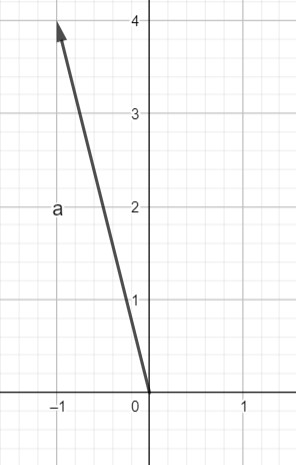
\includegraphics[width = 6cm]{Opgave_11-20/Opgave_20/20.jpg}